% This is an included file. See the master file for more information.
%
% When editing this file:
%
%    1. To change formatting, appearance, or style, please edit openmp.sty.
%
%    2. Custom commands and macros are defined in openmp.sty.
%
%    3. Be kind to other editors -- keep a consistent style by copying-and-pasting to
%       create new content.
%
%    4. We use semantic markup, e.g. (see openmp.sty for a full list):
%         \code{}     % for bold monospace keywords, code, operators, etc.
%         \plc{}      % for italic placeholder names, grammar, etc.
%
%    5. There are environments that provide special formatting, e.g. language bars.
%       Please use them whereever appropriate.  Examples are:
%
%         \begin{fortranspecific}
%         This is text that appears enclosed in blue language bars for Fortran.
%         \end{fortranspecific}
%
%         \begin{note}
%         This is a note.  The "Note -- " header appears automatically.
%         \end{note}
%
%    6. Other recommendations:
%         Use the convenience macros defined in openmp.sty for the minor headers
%         such as Comments, Syntax, etc.
%
%         To keep items together on the same page, prefer the use of
%         \begin{samepage}.... Avoid \parbox for text blocks as it interrupts line numbering.
%         When possible, avoid \filbreak, \pagebreak, \newpage, \clearpage unless that's
%         what you mean. Use \needspace{} cautiously for troublesome paragraphs.
%
%         Avoid absolute lengths and measures in this file; use relative units when possible.
%         Vertical space can be relative to \baselineskip or ex units. Horizontal space
%         can be relative to \linewidth or em units.
%
%         Prefer \emph{} to italicize terminology, e.g.:
%             This is a \emph{definition}, not a placeholder.
%             This is a \plc{var-name}.
%


\section{OMPT}
\label{sec:ompt-overview}

The OMPT interface defines mechanisms for initializing a tool,
exploring the details of an OpenMP implementation, examining OpenMP state
associated with an OpenMP thread, interpreting an OpenMP thread's call stack,
receiving notification about OpenMP \emph{events}, tracing activity on
OpenMP target devices, and controlling a tool from an OpenMP application.

\subsection{Activating a First-Party Tool}
\label{sec:ompt-initialization}

There are three steps to activating a tool. First, an OpenMP
implementation determines whether a tool should be initialized.  If
so, the OpenMP implementation invokes the tool's initializer, enabling
the tool to prepare to monitor the execution on the host. Finally, a
tool may arrange to monitor computation that execute
on target devices. This section explains how the tool and an
OpenMP implementation interact to accomplish these tasks.



\subsubsection{Determining Whether a First-Party Tool Should be Initialized}
\label{sec:ompt-check-tool}

\begin{figure}[h]
  \centering
  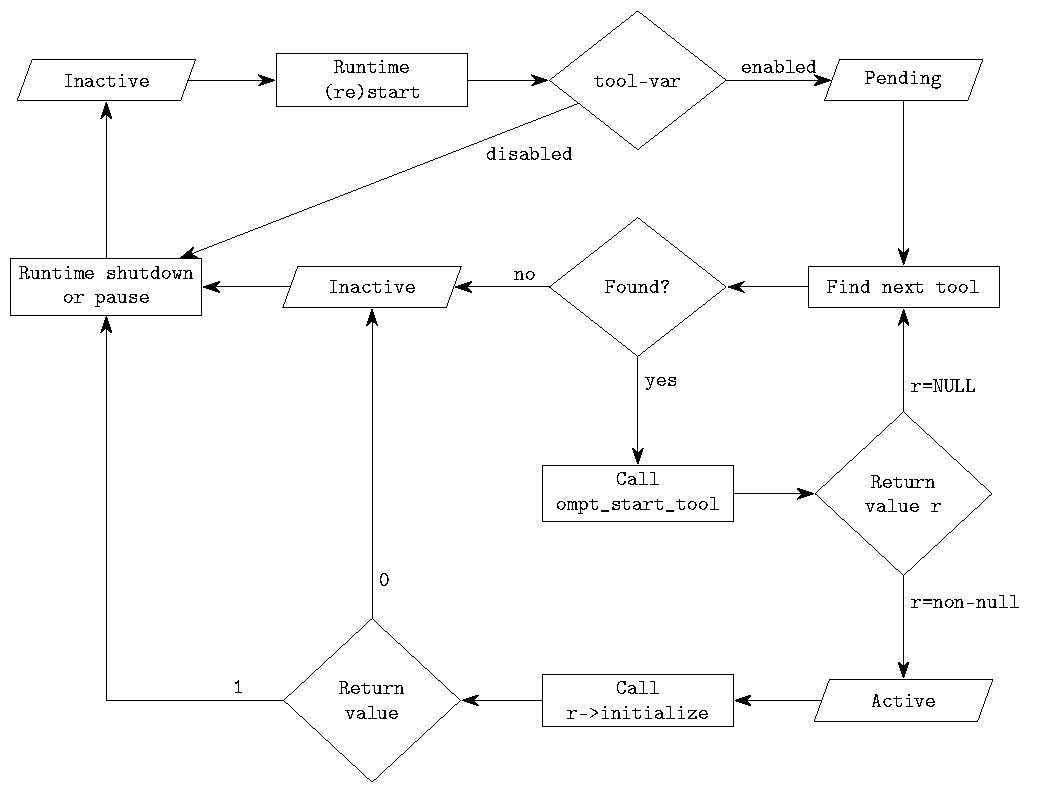
\includegraphics[width=.9\linewidth]{tool_support/ompt_flow_chart.pdf}
  \caption{Flow chart on activating a first-party tool and the states
  of the OMPT interface.}
  \label{fig:ompt_diagram}
\end{figure}

Immediately before an OpenMP implementation initializes itself, it
determines whether it should check for the presence of a tool
interested in using the OMPT interface by examining the \plc{tool-var}
ICV.  If the value of \plc{tool-var} is \plc{disabled}, the OpenMP
implementation will initialize itself without checking whether a
tool is present and the functionality of the OMPT interface will be
unavailable as the program executes.
In this case, the OMPT interface stays \emph{inactive}.

Otherwise, the OMPT interface turns to \emph{pending} and the OpenMP 
implementation tries to find and activate a first-party tool.
There are three ways that a tool can provide this function:

\begin{itemize}
\item statically-linking the tool's definition of \code{ompt_start_tool}
  into an OpenMP application,
\item introducing a dynamically-linked library that includes the tool's definition
  of \code{ompt_start_tool} into the application's address space, or
\item providing the name of a dynamically-loadable library in the 
  \plc{tool-libraries-var} ICV; the library includes
  the tool's definition of \code{ompt_start_tool} and is appropriate
  for the architecture and operating system used by the application.
\end{itemize}

%A tool indicates its interest in using the OMPT interface
%by providing a non-null pointer to an
%\code{ompt_start_tool_result_t}
%structure to an OpenMP implementation as a return value from
%\code{ompt_start_tool}. 

The OpenMP implementation will check to see if a tool has provided an
implementation of \code{ompt_start_tool}.  The OpenMP implementation first
checks if a tool-provided implementation of \code{ompt_start_tool} is
available in the address space, either statically-linked into the
application or in a dynamically-linked library loaded in the address
space. If multiple implementations of \code{ompt_start_tool} are available,
the OpenMP implementation will use the first tool-provided
implementation of \code{ompt_start_tool} found.

If no tool-provided implementation of \code{ompt_start_tool} is found in
the address space, the OpenMP implementation will consult the
\plc{tool-libraries-var} ICV, which contains a (possibly empty) list
of dynamically-linked libraries.  As described in detail in
Section~\ref{sec:OMP_TOOL_LIBRARIES}, the libraries in
\plc{tool-libraries-var}, will be searched for the first usable
implementation of \code{ompt_start_tool} provided by one of the libraries
in the list.

If a tool-provided definition of \code{ompt_start_tool} is found using
either method, the OpenMP implementation will invoke it; if it returns
a non-null pointer to an \code{ompt_start_tool_result_t} structure,
the OMPT interface turns to \emph{active} and can be used by the tool later; 
otherwise the OMPT interface stays \emph{pending} and the implementation 
continues finding another tool.

If no tool can be found, the OMPT interface turns to \emph{inactive}.

Next, the OpenMP implementation will initialize itself. 
If the OMPT interface is \emph{active}, the OpenMP implementation will 
prepare itself for use of the OMPT interface by a tool; 
when the OpenMP implementation is ready to accept calls from the 
first-party tool, it continues with invoking the tool initialization 
as described in the following section.

\crossreferences
\begin{itemize}
\item \plc{tool-libraries-var} ICV, see \specref{sec:Internal Control Variables}.
\item \plc{tool-var} ICV, see \specref{sec:Internal Control Variables}.
\item \code{ompt_start_tool_result_t}, see \specref{sec:ompt_start_tool_result_t}.
\item \code{ompt_start_tool}, see \specref{sec:ompt_start_tool}.
\end{itemize}

\subsubsection{Initializing a First-Party Tool}
\index{tool initialization}
\label{sec:tool-initialize}

If the OMPT interface is active, the OpenMP implementation will invoke 
the tool initializer specified in the \code{ompt_start_tool_result_t} 
structure returned from the \code{ompt_start_tool} function
prior to the occurrence of any OpenMP \emph{event}.

A tool's initializer, described in \specref{sec:ompt_initialize_t}
uses its argument \plc{lookup} to look up pointers
to OMPT interface runtime entry points provided by the OpenMP
implementation; this process is described in \specref{sec:ompt-bind}.
Typically, a tool initializer will first
obtain a pointer to the OpenMP runtime entry point known as
\code{ompt_set_callback} with type signature
\code{ompt_set_callback_t} and then use this runtime entry point to
register tool callbacks for OpenMP events, as described in
\specref{sec:ompt-register-callbacks}.

A tool initializer may use the OMPT interface runtime
entry points known as \code{ompt_enumerate_states} and
\code{ompt_enumerate_mutex_impls}, which have type signatures
\code{ompt_enumerate_states_t} and
\code{ompt_enumerate_mutex_impls_t}, to determine what thread
states and implementations of mutual exclusion a particular OpenMP
implementation employs.

%The descriptions of the enumeration runtime entry point type signatures show how to use them to determine what thread states and mutual exclusion mechanisms an OpenMP implementation supports.

If a tool initializer returns a non-zero value, the OMPT interface 
will stay \emph{active} for the execution; otherwise, the OMPT 
interface turns to \emph{inactive}.

\crossreferences
\begin{itemize}
\item \code{ompt_start_tool_result_t}, see
  \specref{sec:ompt_start_tool_result_t}.
\item \code{ompt_start_tool}, see \specref{sec:ompt_start_tool}.
\item \code{ompt_initialize_t}, see \specref{sec:ompt_initialize_t}.
\item \code{ompt_callback_thread_begin_t}, see \specref{sec:ompt_callback_thread_begin_t}.
\item \code{ompt_enumerate_states_t}, see \specref{sec:ompt_enumerate_states_t}.
\item \code{ompt_enumerate_mutex_impls_t}, see   \specref{sec:ompt_enumerate_mutex_impls_t}.
\item \code{ompt_set_callback_t}, see \specref{sec:ompt_set_callback_t}.
\item \code{ompt_function_lookup_t}, see \specref{sec:ompt_function_lookup_t}.
\end{itemize}


\subsubsubsection{Binding Entry Points in the OMPT Callback Interface}
\label{sec:ompt-bind}

Functions that an OpenMP implementation provides to support the OMPT interface
are not defined as global function symbols. Instead, they are defined as runtime entry points
that a tool can only identify using the \plc{lookup} function provided as an
argument to the tool's initializer. This design avoids tool
implementations that
will fail in certain circumstances when functions defined as part of
the OpenMP runtime are not visible to a tool, even though the tool and
the OpenMP runtime are both present in the same address space.
It also prevents inadvertent use of a tool support routine by
applications.

A tool's initializer receives a function pointer to a \plc{lookup}
runtime entry point with type signature
\code{ompt_function_lookup_t} as its first argument. Using this
function, a tool initializer may obtain a pointer to each of the
runtime entry points that an OpenMP implementation provides to support
the OMPT interface. Once a tool has obtained a
\plc{lookup} function, it may employ it at any point in the future.

For each runtime entry point in the OMPT interface for the host device,
Table~\ref{table:ompt-callback-interface-functions} provides the string
name by which it is known and its associated type signature. Implementations
can provide additional, implementation-specific names and corresponding
entry points as long as they don't use names that start with the prefix
``\code{ompt_}''. These are reserved for future extensions in the
OpenMP specification.

During initialization, a tool should look up each runtime entry point in the
OMPT interface by name and bind a pointer maintained by the tool
that it can use later to invoke the entry point as needed. The entry points
described in Table~\ref{table:ompt-callback-interface-functions}
enable a tool to assess
what thread states and mutual exclusion implementations that an OpenMP runtime supports,
register tool callbacks, inspect callbacks registered,
introspect OpenMP state associated with threads, and use tracing to monitor
computations that execute on target devices.

Detailed information about each runtime entry point listed in
Table~\ref{table:ompt-callback-interface-functions} is included as
part of the description of its type signature.

\crossreferences
\begin{itemize}
\item \code{ompt_enumerate_states_t}, see \specref{sec:ompt_enumerate_states_t}.
\item \code{ompt_enumerate_mutex_impls_t}, see  \specref{sec:ompt_enumerate_mutex_impls_t}.
\item \code{ompt_set_callback_t}, see \specref{sec:ompt_set_callback_t}.
\item \code{ompt_get_callback_t}, see \specref{sec:ompt_get_callback_t}.
\item \code{ompt_get_thread_data_t}, see \specref{sec:ompt_get_thread_data_t}.
\item \code{ompt_get_num_places_t}, see \specref{sec:ompt_get_num_places_t}.
\item \code{ompt_get_place_proc_ids_t}, see \specref{sec:ompt_get_place_proc_ids_t}.
\item \code{ompt_get_place_num_t}, see \specref{sec:ompt_get_place_num_t}.
\item \code{ompt_get_partition_place_nums_t}, see \specref{sec:ompt_get_partition_place_nums_t}.
\item \code{ompt_get_proc_id_t}, see \specref{sec:ompt_get_proc_id_t}.
\item \code{ompt_get_state_t}, see \specref{sec:ompt_get_state_t}.
\item \code{ompt_get_parallel_info_t}, see \specref{sec:ompt_get_parallel_info_t}.
\item \code{ompt_get_task_info_t}, see \specref{sec:ompt_get_task_info_t}.
\item \code{ompt_get_task_memory_t}, see \specref{sec:ompt_get_task_memory_t}.
\item \code{ompt_get_target_info_t}, see \specref{sec:ompt_get_target_info_t}.
\item \code{ompt_get_num_devices_t}, see \specref{sec:ompt_get_num_devices_t}.
\item \code{ompt_get_num_procs_t}, see \specref{sec:ompt_get_num_procs_t}.
\item \code{ompt_get_unique_id_t}, see \specref{sec:ompt_get_unique_id_t}.
\item \code{ompt_finalize_tool_t}, see \specref{sec:ompt_finalize_tool_t}.
\item \code{ompt_function_lookup_t}, see \specref{sec:ompt_function_lookup_t}.
\end{itemize}

\begin{table}[p]
    \caption{OMPT callback interface runtime entry point names and their type signatures.\label{table:ompt-callback-interface-functions}}
    \begin{tabular}{ll}\hline
        {\small \textbf{\textsf{Entry Point String Name}}} & {\small \textbf{\textsf{Type signature}}}\\\hline
        ``{\scode{ompt_enumerate_states}}'' & {\scode{ompt_enumerate_states_t}}\\
        ``{\scode{ompt_enumerate_mutex_impls}}'' & {\scode{ompt_enumerate_mutex_impls_t}}\\
        ``{\scode{ompt_set_callback}}'' & {\scode{ompt_set_callback_t}}\\
        ``{\scode{ompt_get_callback}}'' & {\scode{ompt_get_callback_t}}\\
        ``{\scode{ompt_get_thread_data}}'' & {\scode{ompt_get_thread_data_t}}\\
        ``{\scode{ompt_get_num_places}}'' & {\scode{ompt_get_num_places_t}}\\
        ``{\scode{ompt_get_place_proc_ids}}'' & {\scode{ompt_get_place_proc_ids_t}}\\
        ``{\scode{ompt_get_place_num}}'' & {\scode{ompt_get_place_num_t}}\\
        ``{\scode{ompt_get_partition_place_nums}}'' & {\scode{ompt_get_partition_place_nums_t}}\\
        ``{\scode{ompt_get_proc_id}}'' & {\scode{ompt_get_proc_id_t}}\\
        ``{\scode{ompt_get_state}}'' & {\scode{ompt_get_state_t}}\\
        ``{\scode{ompt_get_parallel_info}}'' & {\scode{ompt_get_parallel_info_t}}\\
        ``{\scode{ompt_get_task_info}}'' & {\scode{ompt_get_task_info_t}}\\
        ``{\scode{ompt_get_task_memory}}'' & {\scode{ompt_get_task_memory_t}}\\
        ``{\scode{ompt_get_num_devices}}'' & {\scode{ompt_get_num_devices_t}}\\
        ``{\scode{ompt_get_num_procs}}'' & {\scode{ompt_get_num_procs_t}}\\
        ``{\scode{ompt_get_target_info}}'' & {\scode{ompt_get_target_info_t}}\\
        ``{\scode{ompt_get_unique_id}}'' & {\scode{ompt_get_unique_id_t}}\\
        ``{\scode{ompt_finalize_tool}}'' & {\scode{ompt_finalize_tool_t}}\\\hline
        % ``{\scode{ompt_callback_device_initialize}}'' & 
        %{\scode{ompt_callback_device_initialize_t}}\\\hline
    \end{tabular}
    
\end{table}

\subsubsection{Monitoring Activity on the Host with OMPT}
\index{event callback registration}
\label{sec:ompt-register-callbacks}

To monitor execution of an OpenMP program on the host device, a tool's
initializer must register to receive notification
of events that occur as an OpenMP program executes.
A tool can register callbacks for OpenMP events using
the runtime entry point known as
\code{ompt_set_callback}.  The possible return codes for
\code{ompt_set_callback} and their meanings are shown in
Table~\ref{table:ToolsSupport_set_rc}.
If the \code{ompt_set_callback} runtime entry point is
called outside a tool's initializer, registration of supported
callbacks may fail with a return code of \code{ompt_set_error}.

All callbacks registered with \code{ompt_set_callback} or returned
by \code{ompt_get_callback} use the dummy type signature
\code{ompt_callback_t}.  While this is a compromise, it is better
than providing unique runtime entry points with a precise type signatures to
set and get the callback for each unique runtime entry point type signature.

Table~\ref{table:valid_rc} indicates the return codes permissible
when trying to register various callbacks. For callbacks where the only registration return code
allowed is \code{ompt_set_always}, an
OpenMP implementation must guarantee that the callback will be
invoked every time a runtime event associated with it occurs. Support
for such callbacks is required in a minimal implementation of the
OMPT interface. For other callbacks where registration is allowed to return values
other than \code{ompt_set_always}, its implementation-defined
whether an OpenMP implementation invokes a registered callback
never, sometimes, or always. If registration for a callback allows
a return code of \code{omp_set_never}, support for invoking such
a callback need not be present in a minimal implementation of the
OMPT interface.  The return code when a callback is
registered enables a tool to know what to expect when the level
of support for the callback can be implementation defined.



\begin{table}
\renewcommand{\arraystretch}{1.2}
\caption{Valid return codes of \code{ompt_set_callback} for each callback.\label{table:valid_rc}}
\begin{tabular}{lp{3em}p{3em}p{3em}p{3em}}
%                                & \rot{\small{\scode{ompt_set_never}}}
%                                & \rot{\small{\scode{ompt_set_sometimes}}
%                                             {\scode{ompt_set_sometimes_paired}}}
%                                & \rot{\small{\scode{ompt_set_always}}}\\
                                \midrule
Return code abbreviation                      & N &S/P& A \\\hline
{\scode{ompt_callback_thread_begin}}          &   &   & * \\
{\scode{ompt_callback_thread_end}}            &   &   & * \\
{\scode{ompt_callback_parallel_begin}}        &   &   & * \\
{\scode{ompt_callback_parallel_end}}          &   &   & * \\
{\scode{ompt_callback_task_create}}           &   &   & * \\
{\scode{ompt_callback_task_schedule}}         &   &   & * \\
{\scode{ompt_callback_implicit_task}}         &   &   & * \\
{\scode{ompt_callback_target}}                 &   &   & * \\
{\scode{ompt_callback_target_data_op}}       &   &   & * \\
{\scode{ompt_callback_target_submit}}         &   &   & * \\
{\scode{ompt_callback_control_tool}}          &   &   & * \\
{\scode{ompt_callback_device_initialize}}     &   &   & * \\
{\scode{ompt_callback_device_finalize}}       &   &   & * \\
{\scode{ompt_callback_device_load}}           &   &   & * \\
{\scode{ompt_callback_device_unload}}         &   &   & * \\
{\scode{ompt_callback_sync_region_wait}}     & * & * & * \\
{\scode{ompt_callback_mutex_released}}        & * & * & * \\
{\scode{ompt_callback_dependences}}          & * & * & * \\
{\scode{ompt_callback_task_dependence}}       & * & * & * \\
{\scode{ompt_callback_work}}                   & * & * & * \\
{\scode{ompt_callback_master}}                 & * & * & * \\
{\scode{ompt_callback_target_map}}            & * & * & * \\
{\scode{ompt_callback_sync_region}}           & * & * & * \\
{\scode{ompt_callback_reduction}}             & * & * & * \\
{\scode{ompt_callback_lock_init}}             & * & * & * \\
{\scode{ompt_callback_lock_destroy}}          & * & * & * \\
{\scode{ompt_callback_mutex_acquire}}         & * & * & * \\
{\scode{ompt_callback_mutex_acquired}}        & * & * & * \\
{\scode{ompt_callback_nest_lock}}             & * & * & * \\
{\scode{ompt_callback_flush}}                  & * & * & * \\
{\scode{ompt_callback_cancel}}                 & * & * & * \\
{\scode{ompt_callback_dispatch}}              & * & * & * \\
\bottomrule
N = {\scode{ompt_set_never}}                   &  \multicolumn{3}{l}{S = {\scode{ompt_set_sometimes}}} \\
P = {\scode{ompt_set_sometimes_paired}}        &  \multicolumn{3}{l}{A = {\scode{ompt_set_always}}} \\
\end{tabular}

\end{table}

To avoid a tool interface specification that enables a tool to
register unique callbacks for an overwhelming number of events,
the interface was collapsed in several ways.
First, in cases where events are naturally paired, e.g., the beginning and
end of a region, and the arguments needed by the callback at each
endpoint were identical, the pair of events was collapsed so that
a tool registers a single callback that will be invoked at both endpoints
with \code{ompt_scope_begin} or \code{ompt_scope_end} provided
as an argument to identify which endpoint the callback invocation reflects.
Second, when a whole class of events is amenable to uniform treatment, only a
single callback is provided for a family of events, e.g.,  a
\code{ompt_callback_sync_region_wait} callback is used for multiple
kinds of synchronization regions, i.e., barrier, taskwait, and taskgroup
regions. Some events involve both kinds of collapsing: the aforementioned
\code{ompt_callback_sync_region_wait} represents
a callback that will be invoked at each endpoint for different kinds
of synchronization regions.


\crossreferences
\begin{itemize}
\item \code{ompt_set_callback_t}, see \specref{sec:ompt_set_callback_t}.
\item \code{ompt_get_callback_t}, see \specref{sec:ompt_get_callback_t}.
\end{itemize}




\subsubsection{Tracing Activity on Target Devices with OMPT}
\index{tracing device activity}
\label{sec:tracing-device-activity}

A target device may or may not initialize a full OpenMP runtime system.
Unless it does, it may not be possible to monitor activity
on a device using a tool interface based on callbacks.
To accommodate such cases, the OMPT interface defines
a monitoring interface for tracing activity on target
devices. Tracing activity on a target device involves the following
steps:

\begin{itemize}
\item To prepare to trace activity on a target device, a tool must register for an
  \code{ompt_callback_device_initialize} callback.  A tool may also register for an
  \code{ompt_callback_device_load} callback to be notified when code is loaded onto a target device or
an \code{ompt_callback_device_unload} callback to be notified when code is unloaded from a target device.
A tool may also optionally register an \code{ompt_callback_device_finalize} callback.
\item When an OpenMP implementation initializes a target device, the
  OpenMP implementation will dispatch the tool's device initialization
  callback on the host device. If the OpenMP implementation or target device does not support tracing,
  the OpenMP implementation will pass a \code{NULL} to the tool's device initializer for its
  \plc{lookup} argument; otherwise, the OpenMP implementation will pass
  a pointer to a device-specific runtime entry point with type
  signature \code{ompt_function_lookup_t} to the tool's device initializer.
\item If the device initializer for the tool receives a
  non-null \plc{lookup} pointer, the tool may use it to query
  which runtime entry points in the tracing interface are available for a target device
  and bind the function pointers returned to tool variables.
  Table~\ref{table:ompt-tracing-interface-functions} indicates the
  names of the runtime entry points that a target device may provide for use
  by a tool.
  Implementations
can provide additional, implementation-specific names and corresponding
entry points as long as they don't use names that start with the prefix
``\code{ompt_}''. Theses are reserved for future extensions in the
OpenMP specification.

  If \plc{lookup} is non-null, the driver for a device will
  provide runtime entry points that enable a tool to control the device's
  interface for collecting traces in its \emph{native} trace format,
  which may be device specific.
  The kinds of trace records available for a device will typically be
  implementation-defined.
  Some devices may also allow a tool to
  collect traces of records in a standard format known as OMPT format,
  described in this document. If so, the \plc{lookup} function will
  return values for the runtime entry points
  \code{ompt_set_trace_ompt} and \code{ompt_get_record_ompt}, which support
  collecting and decoding OMPT traces.
  These runtime entry points are not required for all devices and will only be available for target devices that support
  collection of standard traces in OMPT format.
  For some devices, their native
  tracing format may be OMPT format. In that case, tracing can be
  controlled using either the runtime entry points for native or OMPT
  tracing.

\begin{table}
{\small
\caption{OMPT tracing interface runtime entry point names and their type signatures.\label{table:ompt-tracing-interface-functions}}
\begin{tabular}{ll}\hline
\textbf{\textsf{Entry Point String Name}} & \textbf{\textsf{Type Signature}}\\\hline
``{\scode{ompt_get_device_num_procs}}'' & {\scode{ompt_get_device_num_procs_t}}\\
``{\scode{ompt_get_device_time}}'' & {\scode{ompt_get_device_time_t}}\\
``{\scode{ompt_translate_time}}'' & {\scode{ompt_translate_time_t}}\\
``{\scode{ompt_set_trace_ompt}}'' & {\scode{ompt_set_trace_ompt_t}}\\
``{\scode{ompt_set_trace_native}}'' & {\scode{ompt_set_trace_native_t}}\\
``{\scode{ompt_start_trace}}'' & {\scode{ompt_start_trace_t}}\\
``{\scode{ompt_pause_trace}}'' & {\scode{ompt_pause_trace_t}}\\
``{\scode{ompt_flush_trace}}'' & {\scode{ompt_flush_trace_t}}\\
``{\scode{ompt_stop_trace}}'' & {\scode{ompt_stop_trace_t}}\\
``{\scode{ompt_advance_buffer_cursor}}'' & {\scode{ompt_advance_buffer_cursor_t}}\\
``{\scode{ompt_get_record_type}}'' & {\scode{ompt_get_record_type_t}}\\
``{\scode{ompt_get_record_ompt}}'' & {\scode{ompt_get_record_ompt_t}}\\
``{\scode{ompt_get_record_native}}'' & {\scode{ompt_get_record_native_t}}\\
``{\scode{ompt_get_record_abstract}}'' & {\scode{ompt_get_record_abstract_t}}\\\hline
\end{tabular}
}

\end{table}


\item The tool will use the \code{ompt_set_trace_native}
  and/or the \code{ompt_set_trace_ompt} runtime entry point to specify what
  types of events or activities to monitor on the target device.
  If the \code{ompt_set_trace_native} and/or the
  \code{ompt_set_trace_ompt} runtime entry point is called outside a device
  initializer, registration of supported callbacks may fail with a return code of
  \code{ompt_set_error}.
\item The tool will initiate tracing on the target device by
  invoking \code{ompt_start_trace}. Arguments to \code{ompt_start_trace}
  include two tool callbacks for use by the OpenMP implementation to manage
  traces associated with the target device: one to allocate
  a buffer where the target device can deposit trace events and a
  second to process a buffer of trace events from the target device.
\item When the target device needs a trace buffer, the OpenMP implementation
  will invoke the tool-supplied callback function on the host device to request a new buffer.
\item The OpenMP implementation will monitor execution of OpenMP constructs on the target device as
  directed and record a trace of events or activities into a trace
  buffer. If the device is capable, device trace records will be
  marked with a \plc{host_op_id}---an identifier used to associate
  device activities with the target operation initiated on the host
  that caused these activities.  To correlate activities on the host
  with activities on a device, a tool can register a
  \code{ompt_callback_target_submit} callback.
  Before the host initiates each distinct activity associated with a structured block for a \code{target} construct
  on a target device, the OpenMP implementation will dispatch the \code{ompt_callback_target_submit} callback
  on the host in the thread executing the task that encounters the \code{target} construct.
  Examples of activities that could cause an \code{ompt_callback_target_submit} callback to be dispatched
  include an explicit data copy between a host and target device or execution of a computation.
  This callback provides the tool with a pair of identifiers: one that identifies the target region and a second
  that uniquely identifies an activity associated with that region.
  These identifiers help the tool correlate activities on the target device with their target region.
\item When appropriate, e.g., when a trace buffer fills or needs to be
  flushed, the OpenMP implementation will invoke the tool-supplied buffer
  completion callback to process a non-empty sequence of
  records in a trace buffer associated with the target device.

\item The tool-supplied buffer completion callback may return
  immediately, ignoring records in the trace buffer, or it may iterate
  through them using the \code{ompt_advance_buffer_cursor} entry
  point
  and inspect each one. A tool may inspect the type of the record at
  the current cursor position using the \code{ompt_get_record_type}
  runtime entry point.  A tool may choose to inspect the contents of some or
  all records in a trace buffer using the \code{ompt_get_record_ompt},
  \code{ompt_get_record_native}, or
  \code{ompt_get_record_abstract} runtime entry point.  Presumably, a tool that
  chooses to use the \code{ompt_get_record_native} runtime entry point to
  inspect records will have some knowledge about a device's native
  trace format.  A tool may always use the
  \code{ompt_get_record_abstract} runtime entry point to inspect a trace
  record; this runtime entry point will decode the contents of a native trace record
  and summarize them in a standard format, namely, a
  \code{ompt_record_abstract_t} record.
  Only a record in OMPT format can be retrieved using the
  \code{ompt_get_record_ompt} runtime entry point.
\item Once tracing has been started on a device, a tool may pause or resume
  tracing on the device at any time by invoking
  \code{ompt_pause_trace} with an appropriate flag value as an
  argument.
\item A tool may request that a device flush any pending trace records
  at any time between device initialization and finalization
  by invoking the \code{ompt_flush_trace} runtime entry point for the device.
\item A tool may start or stop tracing on a device at any time using the
  \code{ompt_start_trace} or \code{ompt_stop_trace} runtime entry points,
  respectively. When tracing is stopped on a device, the OpenMP implementation will eventually
  gather all trace records already collected on the device and present to the tool using
  the buffer completion callback provided by the tool.
\item It is legal to shut down an OpenMP implementation while device tracing
is in progress.
\item When an OpenMP implementation begins to shut down, the OpenMP implementation will
  finalize each target device.  Device finalization occurs in three steps.
  First, the OpenMP implementation halts any tracing in progress for the device. Second,
  the OpenMP implementation flushes all trace records collected for the device and presents them to
  the tool using the buffer completion callback associated with that device.
  Finally, the OpenMP implementation dispatches
  any \code{ompt_callback_device_finalize} callback that was previously
  registered by the tool.

\end{itemize}


\crossreferences
\begin{itemize}
\item \code{ompt_callback_device_initialize_t}, see \specref{sec:ompt_callback_device_initialize_t}.
\item \code{ompt_callback_device_finalize_t}, see \specref{sec:ompt_callback_device_finalize_t}.
\item \code{ompt_get_device_num_procs_t}, see \specref{sec:ompt_get_device_num_procs_t}.
\item \code{ompt_get_device_time}, see \specref{sec:ompt_get_device_time_t}.
\item \code{ompt_translate_time}, see \specref{sec:ompt_translate_time_t}.
\item\code{ompt_set_trace_ompt}, see \specref{sec:ompt_set_trace_ompt_t}.
\item \code{ompt_set_trace_native}, see \specref{sec:ompt_set_trace_native_t}.
\item \code{ompt_start_trace}, see \specref{sec:ompt_start_trace_t}.
\item \code{ompt_pause_trace}, see \specref{sec:ompt_pause_trace_t}.
\item \code{ompt_flush_trace}, see \specref{sec:ompt_flush_trace_t}.
\item \code{ompt_stop_trace}, see \specref{sec:ompt_stop_trace_t}.
\item \code{ompt_advance_buffer_cursor}, see \specref{sec:ompt_advance_buffer_cursor_t}.
\item \code{ompt_get_record_type}, see \specref{sec:ompt_get_record_type_t}.
\item \code{ompt_get_record_ompt}, see \specref{sec:ompt_get_record_ompt_t}.
\item \code{ompt_get_record_native}, see \specref{sec:ompt_get_record_native_t}.
\item \code{ompt_get_record_abstract}, see \specref{sec:ompt_get_record_abstract_t}.
\end{itemize}


\subsection{Finalizing a First-Party Tool}
\label{sec:ompt-finalization}

If the OMPT interface is active, the OpenMP implementation will invoke 
the tool finalizer specified in the \code{ompt_start_tool_result_t} 
structure returned from the \code{ompt_start_tool} function
as the OpenMP implementation shuts down.

\crossreferences
\begin{itemize}
\item \code{ompt_finalize_t}, \specref{sec:ompt_finalize_t}
\end{itemize}

\subsection{OMPT Data Types}
\label{sec:ompt-data-types}

\subsubsection{Tool Initialization and Finalization}
\label{sec:ompt_start_tool_result_t}

\summary
A tool's implementation of \code{ompt_start_tool} returns a pointer to an
\code{ompt_start_tool_result_t} structure, which
contains pointers to the tool's
initialization and finalization callbacks as well as an
\code{ompt_data_t} object for use by the tool.


\begin{ccppspecific}
\begin{omptOther}
typedef struct ompt_start_tool_result_t {
  ompt_initialize_t \plc{initialize};
  ompt_finalize_t \plc{finalize};
  ompt_data_t \plc{tool_data};
} ompt_start_tool_result_t;
\end{omptOther}
\end{ccppspecific}


\restrictions

The \plc{initialize} and \plc{finalize} callback pointer values in an
\code{ompt_start_tool_result_t} structure returned by \code{ompt_start_tool} must be
non-null.

\crossreferences
\begin{itemize}
\item \code{ompt_data_t}, see \specref{sec:ompt_data_t}.
\item \code{ompt_finalize_t}, see \specref{sec:ompt_finalize_t}.
\item \code{ompt_initialize_t}, see \specref{sec:ompt_initialize_t}.
\item \code{ompt_start_tool}, see \specref{sec:ompt_start_tool}.
\end{itemize}

\subsubsection{Callbacks}
\label{sec:ompt_callbacks_t}

The following enumeration type indicates the integer codes used to identify
OpenMP callbacks when registering or querying them.


\begin{ccppspecific}
\begin{omptEnum}
typedef enum ompt_callbacks_t {
  ompt_callback_thread_begin             = 1,
  ompt_callback_thread_end               = 2,
  ompt_callback_parallel_begin           = 3,
  ompt_callback_parallel_end             = 4,
  ompt_callback_task_create              = 5,
  ompt_callback_task_schedule            = 6,
  ompt_callback_implicit_task            = 7,
  ompt_callback_target                   = 8,
  ompt_callback_target_data_op           = 9,
  ompt_callback_target_submit            = 10,
  ompt_callback_control_tool             = 11,
  ompt_callback_device_initialize        = 12,
  ompt_callback_device_finalize          = 13,
  ompt_callback_device_load              = 14,
  ompt_callback_device_unload            = 15,
  ompt_callback_sync_region_wait         = 16,
  ompt_callback_mutex_released           = 17,
  ompt_callback_dependences              = 18,
  ompt_callback_task_dependence          = 19,
  ompt_callback_work                     = 20,
  ompt_callback_master                   = 21,
  ompt_callback_target_map               = 22,
  ompt_callback_sync_region              = 23,
  ompt_callback_lock_init                = 24,
  ompt_callback_lock_destroy             = 25,
  ompt_callback_mutex_acquire            = 26,
  ompt_callback_mutex_acquired           = 27,
  ompt_callback_nest_lock                = 28,
  ompt_callback_flush                    = 29,
  ompt_callback_cancel                   = 30,
  ompt_callback_reduction                = 31,
  ompt_callback_dispatch                 = 32
} ompt_callbacks_t;
\end{omptEnum}
\end{ccppspecific}



%\subsubsubsection{Triggers for Miscellaneous Events}
%Most events trigger during the execution of OpenMP directives. Other
%events trigger when an application calls certain runtime library
%routines, e.g., those for setting and unsetting locks.
%This section describes events triggered during initialization and
%finialization of an OpenMP implementation.
%
%\ompteventswithoutdirectives{\code{ompt_callback_thread_begin}}
%\label{sec:ompt_callback_thread_begin}
%
%An OpenMP implementation invokes this callback in the context of an
%initial thread just after it initializes the runtime, or in the
%context of a new thread created by the runtime just after the thread
%initializes itself. In either case, this callback must be the first
%callback for a thread and must occur before the thread executes any
%OpenMP tasks. This callback has type signature
%\code{ompt_callback_thread_begin_t}.  This callback argument
%\code{thread_type} indicates the type of the thread: initial, worker,
%or other.
%
%\ompteventswithoutdirectives{\code{ompt_callback_thread_end}}
%\label{sec:ompt_callback_thread_end}
%
%An OpenMP implementation invokes this callback after an OpenMP thread
%completes all of its tasks but before the thread is destroyed. The
%callback executes in the context of the OpenMP thread. This callback
%must be the last callback event for any worker thread; it is optional
%for other types of threads.  This callback has type signature
%\code{ompt_callback_thread_end_t}.
%
%
%\ompteventswithoutdirectives{\code{ompt_callback_sync_region_wait}}
%\label{sec:ompt_callback_sync_region_wait}
%
%If the \code{ompt_callback_sync_region_wait} callback is registered,
%an OpenMP implementation will invoke this callback when a task starts
%and stops waiting in a barrier region, taskwait region, or taskgroup
%region.  This callback has type signature
%\code{ompt_callback_sync_region_t}.  One region may generate
%multiple pairs of start/stop callbacks if another task is scheduled on
%the thread while the task awaiting completion of the region is
%stalled.  This callback executes in the context of the task that
%encountered the barrier, taskwait, or taskgroup construct.
%
%\ompteventswithoutdirectives{\code{ompt_callback_runtime_shutdown}}
%\label{sec:ompt_callback_runtime_shutdown}
%
%An OpenMP implementation invokes this callback before it shuts down
%the runtime system.  This callback enables a tool to clean up its
%state and record or report information gathered. A runtime may later
%restart and reinitialize the tool by calling the tool initializer
%function (described in Section~\ref{sec:tool-initialize}) again.  This
%callback has type signature \code{ompt_callback_t}.


\subsubsection{Tracing}
\label{sec:ompt-records}

\subsubsubsection{Record Type}

\begin{ccppspecific}
\begin{omptEnum}
typedef enum ompt_record_t {
  ompt_record_ompt               = 1,
  ompt_record_native             = 2,
  ompt_record_invalid            = 3
} ompt_record_t;
\end{omptEnum}
\end{ccppspecific}


\subsubsubsection{Native Record Kind}
\label{sec:ompt_record_native_t}


\begin{ccppspecific}
\begin{omptEnum}
typedef enum ompt_record_native_t {
  ompt_record_native_info  = 1,
  ompt_record_native_event = 2
} ompt_record_native_t;
\end{omptEnum}
\end{ccppspecific}


\subsubsubsection{Native Record Abstract Type}
\label{sec:ompt_record_abstract_t}


\begin{ccppspecific}
\begin{omptRecord}
typedef struct ompt_record_abstract_t {
  ompt_record_native_t \plc{rclass};
  const char *\plc{type};
  ompt_device_time_t \plc{start_time};
  ompt_device_time_t \plc{end_time};
  ompt_hwid_t \plc{hwid};
} ompt_record_abstract_t;
\end{omptRecord}
\end{ccppspecific}


\descr

A \code{ompt_record_abstract_t} record contains several
pieces of information that a tool can use to process a native record
that it may not fully understand. The \plc{rclass} field
indicates whether the record is informational
or represents an event; knowing this can help a tool determine
how to present the record. The record \plc{type} field points to
a statically-allocated, immutable character string that provides
a meaningful name that a tool might want to use to describe the event
to a user. The \plc{start_time} and \plc{end_time} fields are
used to place an event in time. The times are relative to the device
clock. If an event has no associated \plc{start_time} and/or
\plc{end_time}, its value will be
\code{ompt_time_none}. The hardware id field,
\plc{hwid},  is used to indicate the location on the device where
the event occurred. A \plc{hwid} may represent a hardware abstraction
such as a core or a hardware thread id. The meaning of a \plc{hwid}
value for a device is defined by the implementer of the software
stack for the device. If there is no hardware abstraction associated
with the record, the value of \plc{hwid}
will be \code{ompt_hwid_none}.

\subsubsubsection{Record Type}
\label{sec:ompt_record_ompt_t}

\begin{ccppspecific}
\begin{omptRecord}
typedef struct ompt_record_ompt_t {
  ompt_callbacks_t \plc{type};
  ompt_device_time_t \plc{time};
  ompt_id_t \plc{thread_id};
  ompt_id_t \plc{target_id};
  union {
    ompt_record_thread_begin_t \plc{thread_begin};
    ompt_record_idle_t \plc{idle};
    ompt_record_parallel_begin_t \plc{parallel_begin};
    ompt_record_parallel_end_t \plc{parallel_end};
    ompt_record_task_create_t \plc{task_create};
    ompt_record_dependences_t \plc{deps};
    ompt_record_task_dependence_t \plc{task_dep};
    ompt_record_task_schedule_t \plc{task_sched};
    ompt_record_implicit_t \plc{implicit};
    ompt_record_sync_region_t \plc{sync_region};
    ompt_record_target_t \plc{target_record};
    ompt_record_target_data_op_t \plc{target_data_op};
    ompt_record_target_map_t \plc{target_map};
    ompt_record_target_kernel_t \plc{kernel};
    ompt_record_lock_init_t \plc{lock_init};
    ompt_record_lock_destroy_t \plc{lock_destroy};
    ompt_record_mutex_acquire_t \plc{mutex_acquire};
    ompt_record_mutex_t \plc{mutex};
    ompt_record_nest_lock_t \plc{nest_lock};
    ompt_record_master_t \plc{master};
    ompt_record_work_t \plc{work};
    ompt_record_flush_t \plc{flush};
  } \plc{record};
} ompt_record_ompt_t;
\end{omptRecord}
\end{ccppspecific}


\descr
The field \plc{type} specifies the type of record provided by this
structure.
According to the type, event specific information is stored in the matching
\plc{record} entry.
\restrictions
If the \plc{type} is set to \code{ompt_callback_thread_end_t}, the value
of \plc{record} is undefined.

%\begin{note}
%There is no trace record defined for \code{ompt_callback_thread_end_t}, because the thread id is already stored in \code{ompt_record_ompt_t} and the callback signature does not have any further parameters.
%\end{note}

\subsubsection{Miscellaneous Type Definitions}
\label{sec:ompt-types:misc}
This section describes miscellaneous types and enumerations used by the tool interface.

\subsubsubsection{\hcode{ompt_callback_t}}
\label{sec:ompt_callback_t}

Pointers to tool callback functions with many different type
signatures are passed to the \code{ompt_set_callback} runtime entry point and
returned by the \code{ompt_get_callback} runtime entry point. For convenience,
these runtime entry points expect all type signatures to be cast to
a dummy type \code{ompt_callback_t}.


\begin{ccppspecific}
\begin{omptCallback}
typedef void (*ompt_callback_t) (void);
\end{omptCallback}
\end{ccppspecific}


% ompt_id_t

\subsubsubsection{\hcode{ompt_id_t}}
\label{sec:ompt_id_t}
When tracing asynchronous activity on OpenMP devices, tools need identifiers to correlate target regions and operations initiated by the host with
associated activities on a target device. In addition, tools need identifiers to refer to parallel regions and tasks that execute on a device.
OpenMP implementations use identifiers of type \code{ompt_id_t} type for each of these 
purposes.

\begin{ccppspecific}
\begin{omptOther}
typedef uint64_t ompt_id_t;
\end{omptOther}
\end{ccppspecific}

\code{ompt_id_none} is defined as an instance of type \code{ompt_id_t} with the value 0.

Identifiers created on each device must be unique from the time an OpenMP implementation is initialized until it is shut down.
Specifically, this means that (1) identifiers for each target region and target operation instance initiated by the host device must be unique over time on the host,
and (2) identifiers for parallel and task region instances that execute on a device must be unique over time within that device.

Tools should not assume that \code{ompt_id_t} values are small or densely allocated.

% ompt_data_t

\subsubsubsection{\hcode{ompt_data_t}}
\label{sec:ompt_data_t}
Threads, parallel regions, and task regions
each have an associated data object of type \code{ompt_data_t} reserved for use by a tool.
When an OpenMP implementation creates a thread or an instance of a parallel or task region,
it will initialize its associated \code{ompt_data_t} object with the value \code{ompt_data_none}.


\begin{ccppspecific}
\begin{omptOther}
typedef union ompt_data_t {
  uint64_t \plc{value};
  void *\plc{ptr};
} ompt_data_t;
\end{omptOther}
\end{ccppspecific}

\code{ompt_data_none} is defined as an instance of type \code{ompt_data_t} with the data 
and pointer fields equal to 0.

% ompt_device_t

\subsubsubsection{\hcode{ompt_device_t}}
\label{sec:ompt_device_t}
\code{ompt_device_t} is an opaque object representing a device.


\begin{ccppspecific}
\begin{omptOther}
typedef void ompt_device_t;
\end{omptOther}
\end{ccppspecific}




% ompt_device_time_t

\subsubsubsection{\hcode{ompt_device_time_t}}
\label{sec:ompt_device_time_t}
\code{ompt_device_time_t} is an opaque object representing a raw time value from a device.
\label{sec:ompt_time_none}
\code{ompt_time_none} refers to an uknown or unspecified time.


\begin{ccppspecific}
\begin{omptOther}
typedef uint64_t ompt_device_time_t;
\end{omptOther}
\end{ccppspecific}

\code{ompt_time_none} is defined as an instance of type \code{ompt_device_time_t} with 
the value 0.


% ompt_buffer_t

\subsubsubsection{\hcode{ompt_buffer_t}}
\label{sec:ompt_buffer_t}
\code{ompt_buffer_t} is an opaque object handle for a target buffer.


\begin{ccppspecific}
\begin{omptOther}
typedef void ompt_buffer_t;
\end{omptOther}
\end{ccppspecific}




% ompt_buffer_cursor_t

\subsubsubsection{\hcode{ompt_buffer_cursor_t}}
\label{sec:ompt_buffer_cursor_t}
\code{ompt_buffer_cursor_t} is an opaque handle for a position in a target buffer.


\begin{ccppspecific}
\begin{omptOther}
typedef uint64_t ompt_buffer_cursor_t;
\end{omptOther}
\end{ccppspecific}




% ompt_dependence_t

\subsubsubsection{\hcode{ompt_dependence_t}}
\label{sec:ompt_dependence_t}
\code{ompt_dependence_t} is a task dependence.


\begin{ccppspecific}
\begin{omptOther}
typedef struct ompt_dependence_t {
  ompt_data_t \plc{variable};
  ompt_dependence_type_t \plc{dependence_type};
} ompt_dependence_t;
\end{omptOther}
\end{ccppspecific}


\descr
\code{ompt_dependence_t} is a structure to hold information
about a depend clause.
For task dependences, the element \plc{variable} points to the storage location of the 
dependence. 
For doacross dependences, the element \plc{variable} contains the value of a vector 
element, describing 
the dependence.
The element \plc{dependence_type} indicates the type of dependence described.

\crossreferences
\begin{itemize}
\item \code{ompt_dependence_type_t}, see
\specref{sec:ompt_dependence_type_t}.
\end{itemize}


% ompt_thread_t

\subsubsubsection{\hcode{ompt_thread_t}}
\label{sec:ompt_thread_t}
\code{ompt_thread_t} is an enumeration that defines the valid thread type values.


\begin{ccppspecific}
\begin{omptEnum}
typedef enum ompt_thread_t {
  ompt_thread_initial                 = 1,
  ompt_thread_worker                  = 2,
  ompt_thread_other                   = 3,
  ompt_thread_unknown                 = 4
} ompt_thread_t;
\end{omptEnum}
\end{ccppspecific}


Any \plc{initial thread} has thread type \code{ompt_thread_initial}.
All \plc{OpenMP threads} that are not initial threads have thread
type \code{ompt_thread_worker}.  A thread employed by an OpenMP
implementation that does not execute user code has thread type
\code{ompt_thread_other}.  Any thread created outside an OpenMP
implementation that is not an \plc{initial thread} has thread type
\code{ompt_thread_unknown}.

% ompt_scope_endpoint_t

\subsubsubsection{\hcode{ompt_scope_endpoint_t}}
\label{sec:ompt_scope_endpoint_t}
\code{ompt_scope_endpoint_t} is an enumeration that defines valid scope endpoint values.


\begin{ccppspecific}
\begin{omptEnum}
typedef enum ompt_scope_endpoint_t {
  ompt_scope_begin                    = 1,
  ompt_scope_end                      = 2
} ompt_scope_endpoint_t;
\end{omptEnum}
\end{ccppspecific}



% ompt_dispatch_t

\subsubsubsection{\hcode{ompt_dispatch_t}}
\label{sec:ompt_dispatch_t}
\code{ompt_dispatch_t} is an enumeration that defines the valid dispatch kind values.


\begin{ccppspecific}
\begin{omptEnum}
typedef enum ompt_dispatch_t {
  ompt_dispatch_iteration             = 1,
  ompt_dispatch_section               = 2
} ompt_dispatch_t;
\end{omptEnum}
\end{ccppspecific}



% ompt_sync_region_t

\subsubsubsection{\hcode{ompt_sync_region_t}}
\label{sec:ompt_sync_region_t}
\code{ompt_sync_region_t} is an enumeration that defines the valid sync region kind values.


\begin{ccppspecific}
\begin{omptEnum}
typedef enum ompt_sync_region_t {
  ompt_sync_region_barrier                = 1,
  ompt_sync_region_barrier_implicit       = 2,
  ompt_sync_region_barrier_explicit       = 3,
  ompt_sync_region_barrier_implementation = 4,
  ompt_sync_region_taskwait               = 5,
  ompt_sync_region_taskgroup              = 6,
  ompt_sync_region_reduction              = 7
} ompt_sync_region_kind_t;
\end{omptEnum}
\end{ccppspecific}




% ompt_target_data_op_t

\subsubsubsection{\hcode{ompt_target_data_op_t}}
\label{sec:ompt_target_data_op_t}
\code{ompt_target_data_op_t} is an enumeration that defines the valid target data operation values.


\begin{ccppspecific}
\begin{omptEnum}
typedef enum ompt_target_data_op_t {
  ompt_target_data_alloc                = 1,
  ompt_target_data_transfer_to_device   = 2,
  ompt_target_data_transfer_from_device = 3,
  ompt_target_data_delete               = 4,
  ompt_target_data_associate            = 5,
  ompt_target_data_disassociate         = 6
} ompt_target_data_op_t;
\end{omptEnum}
\end{ccppspecific}




% ompt_work_t

\subsubsubsection{\hcode{ompt_work_t}}
\label{sec:ompt_work_t}
\code{ompt_work_t} is an enumeration that defines the valid work type values.


\begin{ccppspecific}
\begin{omptEnum}
typedef enum ompt_work_t {
  ompt_work_loop               = 1,
  ompt_work_sections           = 2,
  ompt_work_single_executor    = 3,
  ompt_work_single_other       = 4,
  ompt_work_workshare          = 5,
  ompt_work_distribute         = 6,
  ompt_work_taskloop           = 7
} ompt_work_t;
\end{omptEnum}
\end{ccppspecific}




% ompt_mutex_t

\subsubsubsection{\hcode{ompt_mutex_t}}
\label{sec:ompt_mutex_t}
\code{ompt_mutex_t} is an enumeration that defines the valid mutex kind values.


\begin{ccppspecific}
\begin{omptEnum}
typedef enum ompt_mutex_t {
  ompt_mutex_lock                     = 1,
  ompt_mutex_nest_lock                = 2,
  ompt_mutex_critical                 = 3,
  ompt_mutex_atomic                   = 4,
  ompt_mutex_ordered                  = 5
} ompt_mutex_t;
\end{omptEnum}
\end{ccppspecific}




% ompt_native_mon_flag_t

\subsubsubsection{\hcode{ompt_native_mon_flag_t}}
\label{sec:ompt_native_mon_flag_t}
\code{ompt_native_mon_flag_t} is an enumeration that defines the valid native monitoring flag values.


\begin{ccppspecific}
\begin{omptEnum}
typedef enum ompt_native_mon_flag_t {
  ompt_native_data_motion_explicit    = 0x01,
  ompt_native_data_motion_implicit    = 0x02,
  ompt_native_kernel_invocation       = 0x04,
  ompt_native_kernel_execution        = 0x08,
  ompt_native_driver                  = 0x10,
  ompt_native_runtime                 = 0x20,
  ompt_native_overhead                = 0x40,
  ompt_native_idleness                = 0x80
} ompt_native_mon_flag_t;
\end{omptEnum}
\end{ccppspecific}




% ompt_task_flag_t

\subsubsubsection{\hcode{ompt_task_flag_t}}
\label{sec:ompt_task_flag_t}
\code{ompt_task_flag_t} is an enumeration that defines the valid task type values.
The least significant byte provides information about the general classification of the task.
The other bits represent properties of the task.

\begin{ccppspecific}
\begin{omptEnum}
typedef enum ompt_task_flag_t {
  ompt_task_initial                   = 0x00000001,
  ompt_task_implicit                  = 0x00000002,
  ompt_task_explicit                  = 0x00000004,
  ompt_task_target                    = 0x00000008,
  ompt_task_undeferred                = 0x08000000,
  ompt_task_untied                    = 0x10000000,
  ompt_task_final                     = 0x20000000,
  ompt_task_mergeable                 = 0x40000000,
  ompt_task_merged                    = 0x80000000
} ompt_task_flag_t;
\end{omptEnum}
\end{ccppspecific}




%xxx
% ompt_task_status

\subsubsubsection{\hcode{ompt_task_status_t}}
\label{sec:ompt_task_status_t}
\code{ompt_task_status_t} is an enumeration that explains the
reasons for switching a task that reached  a task scheduling point.


\begin{ccppspecific}
\begin{omptEnum}
typedef enum ompt_task_status_t {
  ompt_task_complete  = 1,
  ompt_task_yield     = 2,
  ompt_task_cancel    = 3,
  ompt_task_switch    = 4
} ompt_task_status_t;
\end{omptEnum}
\end{ccppspecific}


The value \code{ompt_task_complete} indicates the completion of task that
encountered the task scheduling point. The value \code{ompt_task_yield} indicates
that the task encountered a \code{taskyield} construct. The value \code{ompt_task_cancel} indicates
that the task is canceled due to the encountering of an active cancellation point resulting in the
cancellation of that task.
The value \code{ompt_task_switch} is used in the remaining cases of task switches.

% ompt_target_t

\subsubsubsection{\hcode{ompt_target_t}}
\label{sec:ompt_target_t}
\code{ompt_target_t} is an enumeration that defines the valid target type values.


\begin{ccppspecific}
\begin{omptEnum}
typedef enum ompt_target_t {
  ompt_target                         = 1,
  ompt_target_enter_data              = 2,
  ompt_target_exit_data               = 3,
  ompt_target_update                  = 4
} ompt_target_t;
\end{omptEnum}
\end{ccppspecific}




% ompt_parallel_t

\subsubsubsection{\hcode{ompt_parallel_flag_t}}
\label{sec:ompt_parallel_flag_t}
\code{ompt_parallel_flag_t} is an enumeration that defines the valid invoker values.


\begin{ccppspecific}
\begin{omptEnum}
typedef enum ompt_parallel_flag_t {
  ompt_parallel_invoker_program = 0x00000001,
  ompt_parallel_invoker_runtime = 0x00000002,
  ompt_parallel_league          = 0x40000000,
  ompt_parallel_team            = 0x80000000
} ompt_parallel_flag_t;
\end{omptEnum}
\end{ccppspecific}

\descr

The value \code{ompt_parallel_invoker_program} indicates that on the master thread for a parallel region,
the outlined function associated with implicit tasks for the region
is invoked directly by the application.

The value \code{ompt_parallel_invoker_runtime} indicates that on the master thread for a parallel region, 
the outlined function associated with implicit tasks for the region
is invoked by the runtime.

The value \code{ompt_parallel_league} indicates that the callback indicates
the creation of a league of teams by a \code{teams} construct.

The value \code{ompt_parallel_team} indicates that the callback indicates
the creation of a team of threads by a \code{parallel} construct.





% ompt_target_map_flag_t

\subsubsubsection{\hcode{ompt_target_map_flag_t}}
\label{sec:ompt_target_map_flag_t}
\code{ompt_target_map_flag_t} is an enumeration that defines the valid target map flag values.


\begin{ccppspecific}
\begin{omptEnum}
typedef enum ompt_target_map_flag_t {
  ompt_target_map_flag_to             = 0x01,
  ompt_target_map_flag_from           = 0x02,
  ompt_target_map_flag_alloc          = 0x04,
  ompt_target_map_flag_release        = 0x08,
  ompt_target_map_flag_delete         = 0x10,
  ompt_target_map_flag_implicit       = 0x20
} ompt_target_map_flag_t;
\end{omptEnum}
\end{ccppspecific}




% ompt_dependence_type_t

\subsubsubsection{\hcode{ompt_dependence_type_t}}
\label{sec:ompt_dependence_type_t}
\code{ompt_dependence_type_t} is an enumeration that defines the valid task dependence 
type values.


\begin{ccppspecific}
\begin{omptEnum}
typedef enum ompt_dependence_type_t {
  ompt_dependence_type_in              = 1,
  ompt_dependence_type_out             = 2,
  ompt_dependence_type_inout           = 3,
  ompt_dependence_type_mutexinoutset   = 4,
  ompt_dependence_type_source          = 5,
  ompt_dependence_type_sink            = 6
} ompt_dependence_type_t;
\end{omptEnum}
\end{ccppspecific}





% ompt_cancel_flag_t

\subsubsubsection{\hcode{ompt_cancel_flag_t}}
\label{sec:ompt_cancel_flag_t}
\code{ompt_cancel_flag_t} is an enumeration that defines the valid cancel flag values.


\begin{ccppspecific}
\begin{omptEnum}
typedef enum ompt_cancel_flag_t {
  ompt_cancel_parallel       = 0x01,
  ompt_cancel_sections       = 0x02,
  ompt_cancel_loop           = 0x04,
  ompt_cancel_taskgroup      = 0x08,
  ompt_cancel_activated      = 0x10,
  ompt_cancel_detected       = 0x20,
  ompt_cancel_discarded_task = 0x40
} ompt_cancel_flag_t;
\end{omptEnum}
\end{ccppspecific}


\crossreferences
\begin{itemize}
\item \code{ompt_cancel_t} data type, see \specref{sec:ompt_callback_cancel_t}.
\end{itemize}

% ompt_hwid_t

\subsubsubsection{\hcode{ompt_hwid_t}}
\label{sec:ompt_hwid_t}
\code{ompt_hwid_t} is an opaque object representing a hardware identifier for a target device.
\label{sec:ompt_hwid_none}
\code{ompt_hwid_none} refers to an unknown or unspecified hardware id.
If there is no \code{hwid} associated with a
\code{ompt_record_abstract_t}, the value of \code{hwid} shall be
\code{ompt_hwid_none}.


\begin{ccppspecific}
\begin{omptOther}
typedef uint64_t ompt_hwid_t;
\end{omptOther}
\end{ccppspecific}

\code{ompt_hwid_none} is defined as an instance of type \code{ompt_hwid_t} with the value 
0.



% end miscellaneous types
